\documentclass[12pt,a4paper]{extarticle}
\usepackage{../templates/preamble}

\renewcommand{\typeofnum}{3}
\renewcommand{\papertheme}{Однонаправленные списки.}

\begin{document}
\input{../templates/titlepage.tex}
\setcounter{page}{2}
\tableofcontents
\newpage

% document %
\section{Исходная формулировка задания}
Удалить второй и предпоследний по порядку элементы с заданным значением и удалить весь список.

\section{Определение неясностей}
Если элементов с заданным значением всего 1: он не удаляется, если 2: удаляются оба, 3: только средний.
\section{Контрольный пример}

\begin{tabularx}{\textwidth}{|t|t|}
    \hline
    \multicolumn{1}{|h|}{Ввод} & \multicolumn{1}{h|}{Вывод} \\ \hline
    {\ttfamily\footnotesize\lstinputlisting{files/in.txt}}
    & {\ttfamily\footnotesize\lstinputlisting[firstline=26, lastline=36]{files/out.txt}} \\ \hline
    {\ttfamily\footnotesize\lstinputlisting{files/inq.txt}} & \\ \hline
\end{tabularx}

% \section{Ограничения, обусловленные вычислительным устройством}

\section{Формат файлов}
Входные и выходные файлы для маркерного представления должны иметь следующие форматы:

\begin{xltabular}{\textwidth}{|>{\ttfamily\footnotesize}X|}
    \hline
    \multicolumn{1}{|>{\centering\arraybackslash}X|}{Входные файлы} \\ \hline
    [c...c] \\ \hline

    \multicolumn{1}{|>{\centering\arraybackslash}X|}{Выходные файлы} \\ \hline
    Контрольный вывод:\par
    [с...c\par
    |/]\par
    nullptr\par
    \_\_\_\_\_\_\_\par
    с...c\par
    |/\par
    nullptr\par
    \_\_\_\_\_\_\_\par
    Ответ:
    [с...c\par
    |/]\par
    nullptr\par\\ \hline
\end{xltabular}

\section{Реализация ввода/вывода}
\begin{xltabular}{\textwidth}{|h|s|s|}
    \hline
    \multicolumn{1}{|h|}{Библиотека} &
    \multicolumn{1}{s|}{Ввод} &
    \multicolumn{1}{s|}{Вывод}\\ \hline
    iostream & cin > > & cout < < \\ \hline
    fstream & istream & ostream \\ \hline
\end{xltabular}

\section{Внутреннее представление данных}
\begin{xltabular}{\textwidth}{|
>{\hsize=.2\hsize\centering\arraybackslash\ttfamily\bfseries}X|
>{\hsize=.2\hsize\centering\arraybackslash\itshape}X|
>{\hsize=.6\hsize\centering\arraybackslash}X|
}
\hline
\multicolumn{1}{|>{\hsize=.2\hsize\centering\arraybackslash}X}{Имя переменной} &
\multicolumn{1}{|>{\hsize=.2\hsize\centering\arraybackslash}X}{Тип} &
\multicolumn{1}{|>{\hsize=.6\hsize\centering\arraybackslash}X|}{Описание} \\ \hline
in & ifstream & Входной файл \\ \hline
inQ & ifstream & Входной файл цели \\ \hline
out & ofstream & Выходной файл \\ \hline
l, q & list & Списки \\ \hline
\end{xltabular}

Структура {\ttfamily\bfseries strL} (из {\ttfamily strL.hpp}):
\begin{xltabular}{\textwidth}{|
>{\hsize=.2\hsize\centering\arraybackslash\ttfamily\bfseries}X|
>{\hsize=.1\hsize\centering\arraybackslash\itshape}X|
>{\hsize=.7\hsize\centering\arraybackslash}X|}
\hline
\multicolumn{1}{|>{\hsize=.2\hsize\centering\arraybackslash}X}{Имя аргумента} &
\multicolumn{1}{|>{\hsize=.1\hsize\centering\arraybackslash}X}{Тип} &
\multicolumn{1}{|>{\hsize=.7\hsize\centering\arraybackslash}X|}{Описание} \\ \hline
chars & char* & Символы строки \\ \hline
chars\_c & unsigned & Длина строки \\ \hline
\end{xltabular}

Структура {\ttfamily\bfseries L1} (из {\ttfamily L1.hpp}):
\begin{xltabular}{\textwidth}{|
>{\hsize=.2\hsize\centering\arraybackslash\ttfamily\bfseries}X|
>{\hsize=.1\hsize\centering\arraybackslash\itshape}X|
>{\hsize=.7\hsize\centering\arraybackslash}X|}
\hline
\multicolumn{1}{|>{\hsize=.2\hsize\centering\arraybackslash}X}{Имя аргумента} &
\multicolumn{1}{|>{\hsize=.1\hsize\centering\arraybackslash}X}{Тип} &
\multicolumn{1}{|>{\hsize=.7\hsize\centering\arraybackslash}X|}{Описание} \\ \hline
val & strL & Информация \\ \hline
next & L1 * & Следующий нод \\ \hline
\end{xltabular}
Структура {\ttfamily\bfseries list} (из {\ttfamily L1.hpp}):
\begin{xltabular}{\textwidth}{|
>{\hsize=.2\hsize\centering\arraybackslash\ttfamily\bfseries}X|
>{\hsize=.1\hsize\centering\arraybackslash\itshape}X|
>{\hsize=.7\hsize\centering\arraybackslash}X|}
\hline
\multicolumn{1}{|>{\hsize=.2\hsize\centering\arraybackslash}X}{Имя аргумента} &
\multicolumn{1}{|>{\hsize=.1\hsize\centering\arraybackslash}X}{Тип} &
\multicolumn{1}{|>{\hsize=.7\hsize\centering\arraybackslash}X|}{Описание} \\ \hline
first, last & L1 * & Первый и последний нод \\ \hline
first\_prev, cur\_prev & L1 * & Предыдущие первому и текущему ноду \\ \hline
\end{xltabular}

\section{Описание функций}
\subsection{strL.сpp}
\subsubsection{Параметры}
\begin{xltabular}
    {\textwidth}{|X|X|X|X|X|X|}
    \hline
    \multirow{2}{0.14\textwidth}{\centering Имя функции} &
    \multicolumn{4}{c|}{Параметры} &
    \multirow{2}{0.14\textwidth}{\centering Возращаемый тип} \\ \cline{2-5}
    & Входные & Выходные & Модифицир. & Транзитные & \\ \hline
    strL::init & char *\_chars, int \_chars\_c & & & & strL \& \\ \hline
    strL::print & ostream\& out & & out & & void \\ \hline
    strL::destroy & & & & & void \\ \hline
\end{xltabular}

\subsubsection{Функции}
\begin{listed}
    \item strL::init Инициализирует строку.
    \item strL::print Выводит строку в поток.
    \item strL::destroy Удаляет строку с освобождением памяти.
\end{listed}
\subsection{files.сpp}
\subsubsection{Параметры}
\begin{xltabular}
    {\textwidth}{|X|X|X|X|X|X|}
    \hline
    \multirow{2}{0.14\textwidth}{\centering Имя функции} &
    \multicolumn{4}{c|}{Параметры} &
    \multirow{2}{0.14\textwidth}{\centering Возращаемый тип} \\ \cline{2-5}
    & Входные & Выходные & Модифицир. & Транзитные & \\ \hline
    readfile & istream\& in & & in & & list \& \\ \hline
    bar & ostream\& out & & out & & void \\ \hline
\end{xltabular}

\subsubsection{Функции}
\begin{listed}
    \item readfile Читает файл.
    \item bar Выводит полоску в поток.
\end{listed}
\subsection{L1.сpp}
\subsubsection{Параметры}
\begin{xltabular}
    {\textwidth}{|X|X|X|X|X|X|}
    \hline
    \multirow{2}{0.14\textwidth}{\centering Имя функции} &
    \multicolumn{4}{c|}{Параметры} &
    \multirow{2}{0.14\textwidth}{\centering Возращаемый тип} \\ \cline{2-5}
    & Входные & Выходные & Модифицир. & Транзитные & \\ \hline
    list::init\_list & & & & & void \\ \hline
    list::destroy\_list & & & & & void \\ \hline
    list::is\_empty & & & & & bool \\ \hline
    list::push\_back & strL \_val & & & & void \\ \hline
    list::print & ostream\& out & & out & & void \\ \hline
    list::count\_elem & strL str & & & str & int  \\ \hline
    list::find\_prev & strL \_val & & & & L1 *  \\ \hline
    list::remove\_next & L1 *node & & node & & void \\ \hline
    process & list \&l, list q, int count & & l & q & void \\ \hline
\end{xltabular}


\subsubsection{Функции}
\begin{listed}
    \item list::init\_list Инициализирует список.
    \item list::destroy\_list Освобождает память нодов.
    \item list::is\_empty Проверяет, пустой ли список.
    \item list::push\_back Пихает элемент в конец.
    \item list::print Выводит список стрелочкой.
    \item list::count\_elem подсчитывает количество заданного элемента.
    \item list::find\_prev Ищет нод, следующий за которым имеет заданное значение.
    \item list::remove\_next Удаляет следующий нод.
    \item process Выполнение задачи.
\end{listed}

\section{Описание алгоритма}
После считывания списка, считается количество заданных элементов в списке. Если их 1 --- ничего не делаем,
2 --- удаляем в обратном порядке, любое другое количество --- пропускаем первое вхождение, запоминмаем второе и последнее и
итериремся, сдвигая последнее в предыдущее по всем элементам списка, потом удаляем элементы.

{\centering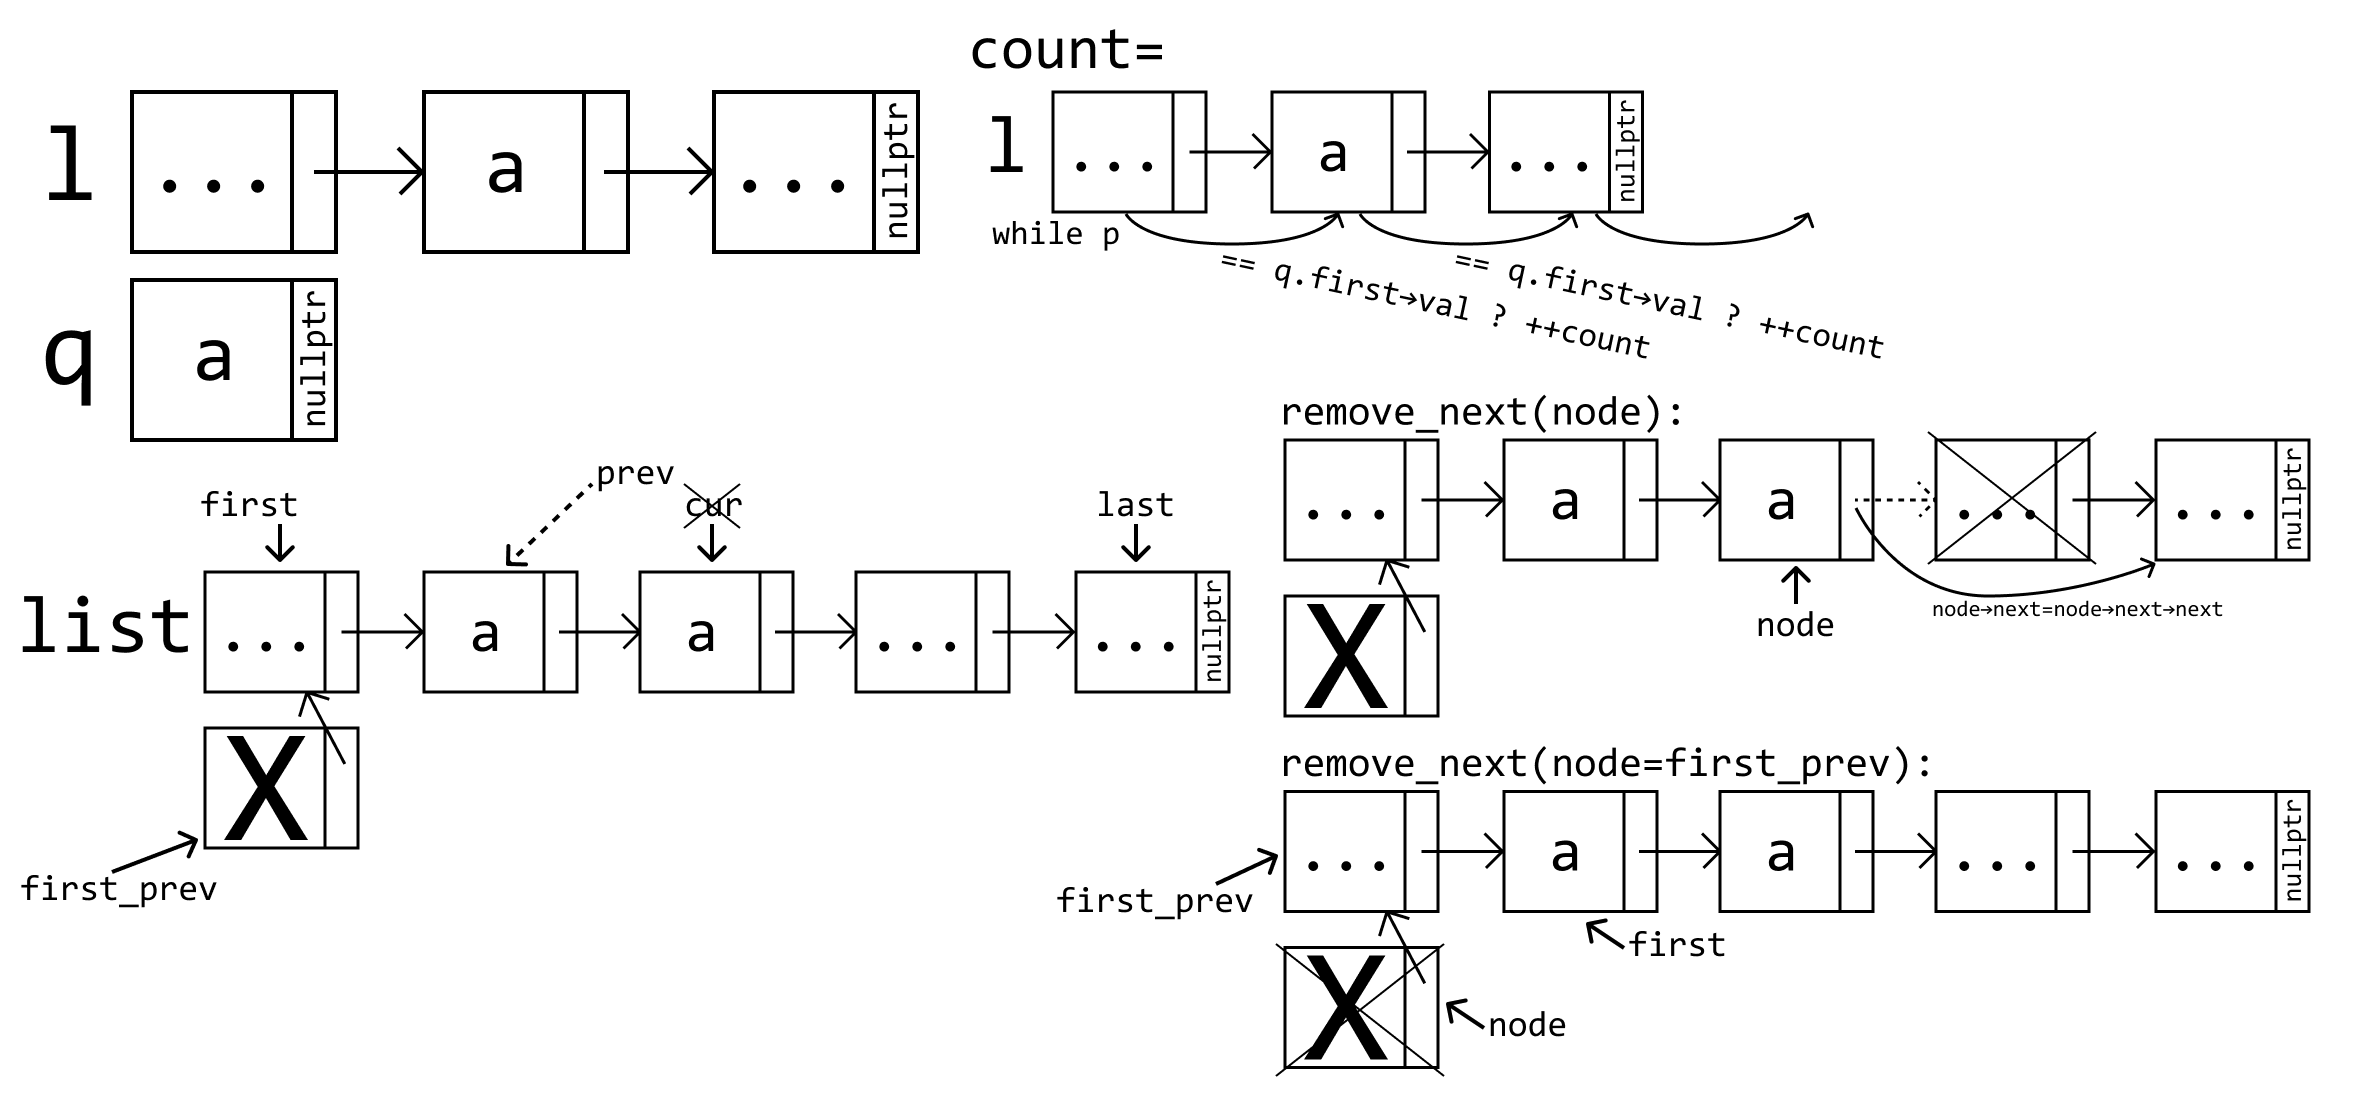
\includegraphics[width=\linewidth]{figures/Frame 14.png}}

Ниже представлены блок-схемы интересных функций.

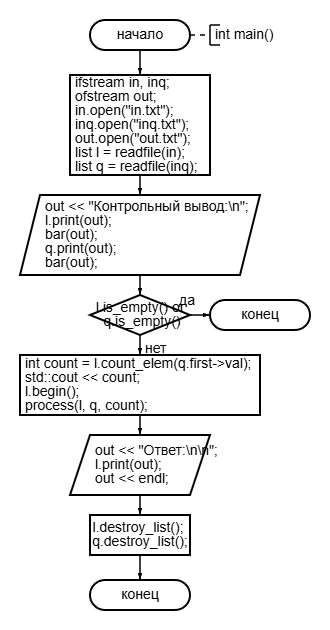
\includegraphics[width=0.33\linewidth]{figures/main.png}
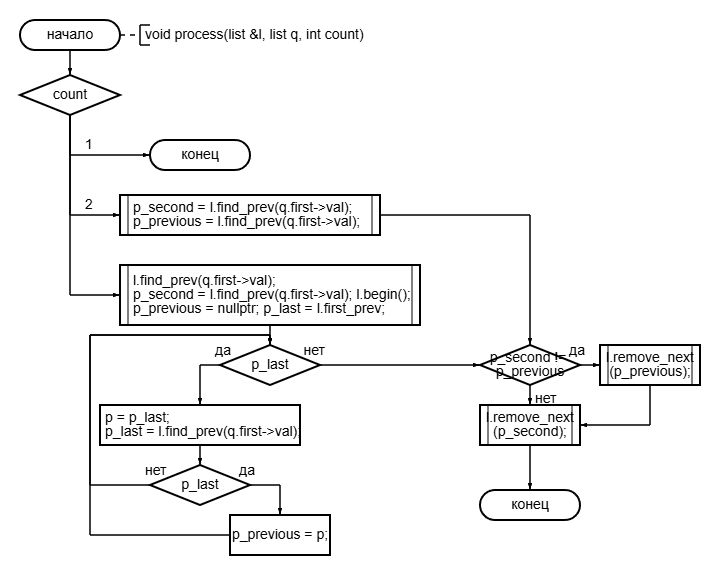
\includegraphics[width=0.33\linewidth]{figures/process.png}
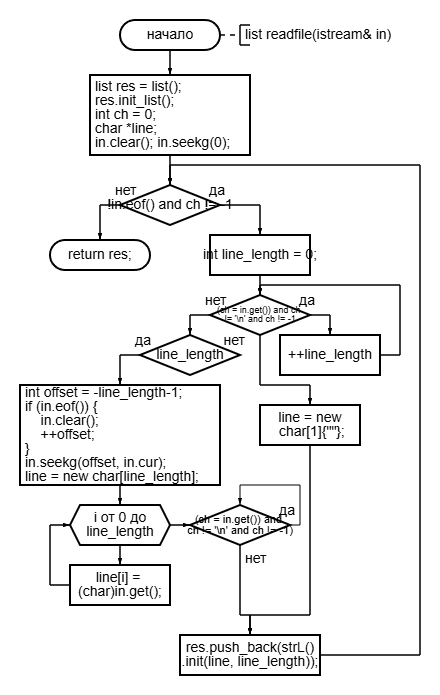
\includegraphics[width=0.33\linewidth]{figures/readfile.png}

\section{Исходный код программы}

\begin{xltabular}
    {\textwidth}{X|X}
    strL.hpp: \lstinputlisting[language=C++]{../../tasks/3/headers/strL.hpp} &
    strL.cpp: \lstinputlisting[language=C++]{../../tasks/3/modules/strL.cpp} \\
\end{xltabular}
\begin{xltabular}
    {\textwidth}{X|X}
    files.hpp: \lstinputlisting[language=C++]{../../tasks/3/headers/files.hpp} &
    files.cpp: \lstinputlisting[language=C++]{../../tasks/3/modules/files.cpp} \\
\end{xltabular}
\begin{xltabular}
    {\textwidth}{X|X}
    L1.hpp: \lstinputlisting[language=C++]{../../tasks/3/headers/L1.hpp} &
    L1.cpp: \lstinputlisting[language=C++, lastline=70]{../../tasks/3/modules/L1.cpp} \\
\end{xltabular}
\lstinputlisting[language=C++]{../../tasks/3/main.cpp}
\begin{center}
    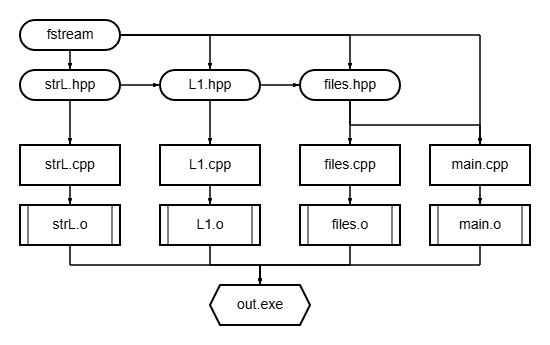
\includegraphics[width=0.5\textwidth]{figures/chart.png}
\end{center}

\section{Результаты работы программы}
\begin{tabularx}{\textwidth}{|>{\ttfamily\footnotesize}X|>{\ttfamily\footnotesize}X|}
    \hline
    \multicolumn{2}{|X|}{Ввод} \\ \hline
    \multicolumn{2}{|X|}{\lstinputlisting{files/in.txt}\par\lstinputlisting{files/inq.txt}} \\ \hline
    \multicolumn{2}{|X|}{Вывод} \\ \hline
    \multicolumn{2}{|X|}{\lstinputlisting{files/out.txt}} \\ \hline
\end{tabularx}

\section{Вывод о проделанной работе}
В ходе выполнения работы я научился работе с однонаправленными списками, удалению элементов, представлению
списка по предыдущим элементам и узнал и включил в работу использование формуляров списка.

\end{document}
